%%%%%%%%%%%%%%%%%%%%%%%%%%%%%%%%%%%
%This is the LaTeX ARTICLE template for RSC journals
%Copyright The Royal Society of Chemistry 2016
%%%%%%%%%%%%%%%%%%%%%%%%%%%%%%%%%%%

\documentclass[9pt]{article}
\usepackage{extsizes}
\usepackage[super,sort&compress,comma]{natbib} 
\usepackage[version=3]{mhchem}
\usepackage[left=1.5cm, right=1.5cm, top=1.785cm, bottom=2.0cm]{geometry}
\usepackage{balance}
\usepackage{times,mathptmx}
\usepackage{sectsty}
\usepackage{graphicx} 
\usepackage{lastpage}
\usepackage[format=plain,justification=justified,singlelinecheck=false,font={stretch=1.125,small,sf},labelfont=bf,labelsep=space]{caption}
\usepackage{float}
\usepackage{fancyhdr}
\usepackage{fnpos}
\usepackage{siunitx}
\usepackage[english]{babel}
\addto{\captionsenglish}{%
  \renewcommand{\refname}{Notes and references}
}
\usepackage{array}
\usepackage{droidsans}
\usepackage{charter}
\usepackage[T1]{fontenc}
\usepackage[usenames,dvipsnames]{xcolor}
\usepackage{setspace}
\usepackage[compact]{titlesec}
\usepackage{hyperref}
%%%Please don't disable any packages in the preamble, as this may cause the template to display incorrectly.%%%

\usepackage{todonotes}

\usepackage{epstopdf}%This line makes .eps figures into .pdf - please comment out if not required.

\definecolor{cream}{RGB}{222,217,201}

\begin{document}

\pagestyle{fancy}
\thispagestyle{plain}
\fancypagestyle{plain}{

%%%HEADER%%%
\fancyhead[C]{
\includegraphics[width=18.5cm]{head_foot/header_bar}}
\fancyhead[L]{\hspace{0cm}\vspace{1.5cm}
\includegraphics[height=30pt]{head_foot/journal_name}}
\fancyhead[R]{\hspace{0cm}\vspace{1.7cm}
\includegraphics[height=55pt]{head_foot/RSC_LOGO_CMYK}}
\renewcommand{\headrulewidth}{0pt}
}
%%%END OF HEADER%%%

%%%PAGE SETUP - Please do not change any commands within this section%%%
\makeFNbottom
\makeatletter
\renewcommand\LARGE{\@setfontsize\LARGE{15pt}{17}}
\renewcommand\Large{\@setfontsize\Large{12pt}{14}}
\renewcommand\large{\@setfontsize\large{10pt}{12}}
\renewcommand\footnotesize{\@setfontsize\footnotesize{7pt}{10}}
\makeatother

\renewcommand{\thefootnote}{\fnsymbol{footnote}}
\renewcommand\footnoterule{\vspace*{1pt}% 
\color{cream}\hrule width 3.5in height 0.4pt \color{black}\vspace*{5pt}} 
\setcounter{secnumdepth}{5}

\makeatletter 
\renewcommand\@biblabel[1]{#1}            
\renewcommand\@makefntext[1]% 
{\noindent\makebox[0pt][r]{\@thefnmark\,}#1}
\makeatother 
\renewcommand{\figurename}{\small{Fig.}~}
\sectionfont{\sffamily\Large}
\subsectionfont{\normalsize}
\subsubsectionfont{\bf}
\setstretch{1.125} %In particular, please do not alter this line.
\setlength{\skip\footins}{0.8cm}
\setlength{\footnotesep}{0.25cm}
\setlength{\jot}{10pt}
\titlespacing*{\section}{0pt}{4pt}{4pt}
\titlespacing*{\subsection}{0pt}{15pt}{1pt}
%%%END OF PAGE SETUP%%%

%%%FOOTER%%%
\fancyfoot{}
\fancyfoot[LO,RE]{\vspace{-7.1pt}
\includegraphics[height=9pt]{head_foot/LF}}
\fancyfoot[CO]{\vspace{-7.1pt}\hspace{13.2cm}
\includegraphics{head_foot/RF}}
\fancyfoot[CE]{\vspace{-7.2pt}\hspace{-14.2cm}
\includegraphics{head_foot/RF}}
\fancyfoot[RO]{\footnotesize{\sffamily{1--\pageref{LastPage} ~\textbar  \hspace{2pt}\thepage}}}
\fancyfoot[LE]{\footnotesize{\sffamily{\thepage~\textbar\hspace{3.45cm} 1--\pageref{LastPage}}}}
\fancyhead{}
\renewcommand{\headrulewidth}{0pt} 
\renewcommand{\footrulewidth}{0pt}
\setlength{\arrayrulewidth}{1pt}
\setlength{\columnsep}{6.5mm}
\setlength\bibsep{1pt}
%%%END OF FOOTER%%%

%%%FIGURE SETUP - please do not change any commands within this section%%%

\graphicspath{{Figures/}}

\makeatletter 
\newlength{\figrulesep} 
\setlength{\figrulesep}{0.5\textfloatsep} 

\newcommand{\topfigrule}{\vspace*{-1pt}% 
\noindent{\color{cream}\rule[-\figrulesep]{\columnwidth}{1.5pt}} }

\newcommand{\botfigrule}{\vspace*{-2pt}% 
\noindent{\color{cream}\rule[\figrulesep]{\columnwidth}{1.5pt}} }

\newcommand{\dblfigrule}{\vspace*{-1pt}% 
\noindent{\color{cream}\rule[-\figrulesep]{\textwidth}{1.5pt}} }

\makeatother
%%%END OF FIGURE SETUP%%%

%%%TITLE, AUTHORS AND ABSTRACT%%%
\twocolumn[
  \begin{@twocolumnfalse}
\vspace{3cm}
\sffamily
\begin{tabular}{m{4.5cm} p{13.5cm} }

  
\includegraphics{head_foot/DOI} & \noindent\LARGE{\textbf{This is the title$^\dag$}} \\
  % Article title goes here instead of the text "This is the title"
  \vspace{0.3cm} & \vspace{0.3cm} \\

                                  & \noindent\large{Full Name,$^{\ast}$\textit{$^{a}$} Full Name,\textit{$^{b\ddag}$} and Full Name\textit{$^{a}$}} \\
                                  % Author names go here instead of "Full name", etc.

  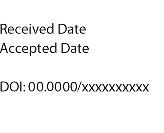
\includegraphics{head_foot/dates} & \noindent\normalsize{The abstract should be a single paragraph
                                      which summarises the content of the article. Any references in
                                      the abstract should be written out in full
                                      \textit{e.g.}\ [Surname \textit{et al., Journal Title}, 2000,
                                      \textbf{35}, 3523].} \\
                                    % The abstrast goes here instead of the text "The abstract should be..."

\end{tabular}

\end{@twocolumnfalse} \vspace{0.6cm}

]
%%% END OF TITLE, AUTHORS AND ABSTRACT%%%

%%% FONT SETUP - please do not change any commands within this section
\renewcommand*\rmdefault{bch}\normalfont\upshape \rmfamily
\section*{}
\vspace{-1cm}


%%% FOOTNOTES%%%

\footnotetext{\textit{$^{a}$~Address, Address, Town, Country. Fax: XX XXXX XXXX;
    Tel: XX XXXX XXXX; E-mail: xxxx@aaa.bbb.ccc}}
\footnotetext{\textit{$^{b}$~Address, Address, Town, Country. }}

% Please use \dag to cite the ESI in the main text of the article. If you
% article does not have ESI please remove the the \dag symbol from the title and
% the footnotetext below.
\footnotetext{\dag~Electronic Supplementary Information (ESI) available:
  [details of any supplementary information available should be included here].
  See DOI: 00.0000/00000000.}
% additional addresses can be cited as above using the lower-case letters, c, d,
% e... If all authors are from the same address, no letter is required

\footnotetext{\ddag~Additional footnotes to the title and authors can be
  included \textit{e.g.}\ `Present address:' or `These authors contributed
  equally to this work' as above using the symbols: \ddag, \textsection, and \P.
  Please place the appropriate symbol next to the author's name and include a
  \texttt{\textbackslash footnotetext} entry in the the correct place in the
  list.}


%%%END OF FOOTNOTES%%%

%%%MAIN TEXT%%%%
\onecolumn
\doublespacing

\thispagestyle{fancy}

\section{Introduction}
The cell is a highly complex unit present in all living organisms: it continues
the building block of life. Essentially, consists of a closed domain containing
smaller organelles in a highly complex and crowded aqueous solution, all
enclosed by a bilayer made of mainly pospholipids and containing fatty acids,
sugars, cholesterol and proteins, among others. This bilayer is called cell
membrane or cytoplasmic membrane. Membranes itself are very complex molecular
organizations with variable and inhomogeneous composition, and its atomic level
understanding is a very difficult task. For this reason, the employment o9f
membrane mimetics and models has become common practice.\todo{Cita 1}\\

Membrane proteins play a significant role in human pathologies \todo{Cita 2 y
  3}. About 30\% of human genes code por membrane proteins \todo{cita 4} and
they are targeted by more than 50\% of drugs \todo{cita 5 y 6}. Therefore, most
drugs have to cross membrane interfaces to reach their active site, and
consequently, the activity of these drugs depends, among other factors, on their
ability to perform this task. This is particularly true for local anesthetics
(LA). For more than hundred years it has been observed that the effectiveness of
many LA correlates positively with lipophilicity \todo{cita 7-10}, showing the
importance of becoming incorporated into the bilayer. It is widely accepted that
inhibition of voltage gated \ce{Na+} channels are directly involved in the
mechanism of LA\todo{cita 11 y 12} and three possible pictures have been
proposed: (a) LA directly binds the pore of the channel blocking the transit of
ions, (b) LA reaches the active site by one of the lateral cavities filled with
hydrophobic membrane components, and (c) the presence of LA near the interface
modifies the structure and dynamics of the bilayer itself, perturbing the
channel conformational dynamics and functioning\todo{cita de 13 a 21}. Despite
which mechanisms are actually taking place, crossing membrane interfaces to
become incorporated into the hydrophobic domain appears to be a crucial step for
most drugs.\\

Benzocaine is a well known LA for topical use. It has been widely employed
anesthetizing the oropharynx for trans-esophageal echocardiography, bonchoscopy,
esophagogastroduodenoscopy, in cold sores, mouth ulcers, toothache, sore gums
and denture ache among others\todo{cita 22}. A significant number of cases of BZ
induced cyanosis (methemoglobinemia) have been reported along the
years\todo{cita 23}, however it still remain in use.\\

Benzocaine has been subject of a significant number of studies, including free energy
transfer from water to the interior of different membrane mimetics \todo{cita
  24-27}, estimations about location and orientation in different bilayers and
monolayers\todo{cita 28-32}, interactions with a variety of solvents\todo{cita
  33-37}, encapsulation in different structures for controlled delivery
purposes\todo{cita 38-42} among others. All the evidence confirms that Benzocaine is
able to cross the interface of membrane mimetics to become incorporated into the
hydrophobic bilayer to finally be located at the inner interface.\\

Contrary to most LA, Levodopa (or L-DOPA), the precursor of the neurotransmitter
dopamine, commonly used in treatment of Parkinson's disease, is able to cross
membrane interfaces only via active processes\todo{cita 43}. Theres is evidence
that neurotransmitters may function as anesthetics and it is postulated that
they share the passive mechanism (c) mentioned above for LA\todo{cita 44}.
Therefore, in the absence of appropriate specific receptors, Levodopa should
remain attached to
the outer interface and not reach the hydrophobic bilayer\todo{cita 45}.\\
In this article, we developed a new nematic lyotropic liquid crystal, with
bilayer structure, susceptible to be used as membrane mimetic. It is made of
sodium dodecyl sulfate (SDS), 1-decanol (DeOH), sodium sulphate (\ce{Na2O4}) and
a mixture of natural phospholipids extracted from soybean, all dissolved in
water. The anionic mesophase was characterized using polarized light microscopy
textures and $^2$H-NMR quadrupole splittings. To test the capability of the new
mimetic to reproduce cellular membrane behavior, Benzocaine and Levodopa were
dissolved in the mesophase solution. According to previous evidence, Benzocaine
should spontaneously be incorporated inside the bilayer and become located
around the inner interface, whereas Levodopa should remain attached to the outer
interface. To observe experimentally the bilayer dynamical behavior and
interactions, $^2$H-NMR quadrupole splittings from HDO, DeOH-$\alpha$-d$_2$ and
SDS-d$_{25}$ were measured. Besides, to test for Benzocaine and Levodopa
location and dynamics, splittings from Benzocaine-d$_4$ and Levodopa-d$_3$ were
also measured. To obtain a more detailed characterization of the bilayer
interface and information about location, orientation, dynamics and interactions
of Benzocaine and Levodopa with the bilayer components, the experimental
measurements were complemented with classical molecular dynamics (MD)
simulations. The results show that prevous observations on Benzocaine and
Levodopa dissolved in different membrane mimetics are reproduced in this case,
reaffirming the membrane mimetic character of the new mesophase.

\section{Preparation of the membrane mimetic}

The reagents SDS, SDS-d$_{25}$, sodium sulphate and the phospholipid mixture
were purchased from \textit{Sigma Aldrich}. DeOH, deuterium oxide and HPLC-grade
water were purchased from \textit{Merck}. All these reagents were employed
without alterations, excepting sodium sulphate which was oven dried 24 hours
before use.
Deuterated 1-decanol (DeOH-$\alpha$-d$_2$) was synthesized by reducing ethyl
decanoate (\ce{C12G24O2}) with lithium aluminum deuteride (\ce{LiAlD4}) and
purified by vacuum fractional distillation.\\

\begin{figure}[h]
\centering
  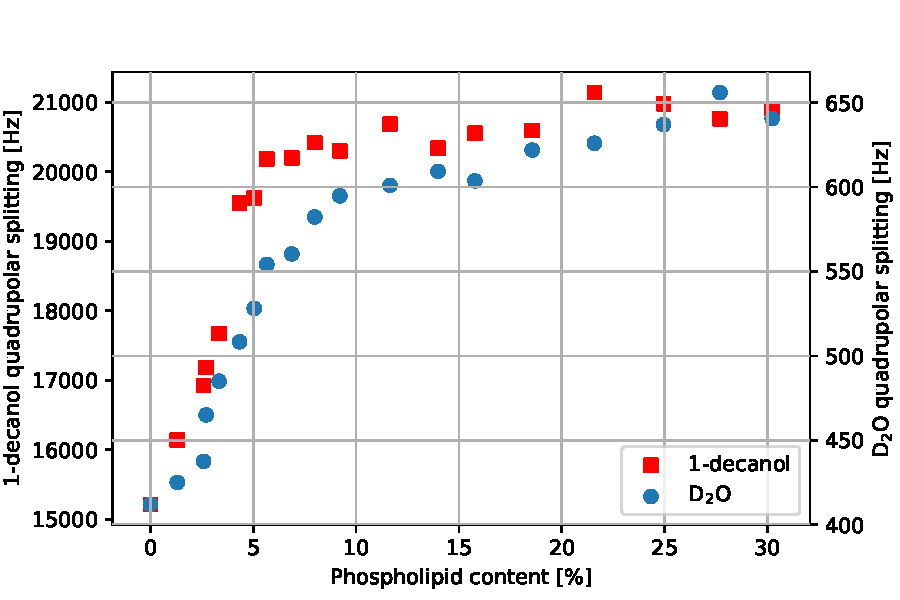
\includegraphics[width=\columnwidth]{splitting_v_phospholipid}
  \caption{Quadrupolar splittings of 1-decanol-$\alpha$-$d_2$ and \ce{D2O} in
    $^2$H-RMN as a function of the phospholipid content in the mimetic.}
  \label{fig:1st_max}
\end{figure}

In order to achieve a membrane mimetic that behaves as similar as possible to
the actual cellular membrane, it is necessary to maximize its phospholipid
concentration. This is important considering that multiple researchers have
concluded that there are specific interactions between the phosphate from the
multiple phospholipids and certain amino-acids that modify the membrane
permeability where this interaction occurs\todo{citar esto}.\\
Also, the membrane mimetic must orient itself in presence of an external
magnetic field. This is so the deuterated probes in the mimetic can produce a
\textit{quadrupole splitting} in its $^2$H-RMN spectrum, which will be used to
assess the mobility and orientation of each deuterium labeled component.\\
Both these requirements were fulfilled by employing the membrane mimetic
developed by Bahamondes \textit{et al}\todo{citar al victor} as starting point,
then introducing and maximizing a concentration of phospholipid onto this
composition. The maximization was performed in two steps. In a first step, a
batch of membrane mimetics was prepared, each one with an increasing amount of
phospholipid from 0\% up to 30\% (see figure \ref{fig:1st_max}), $^2$H-RMN
spectra and polarized light microscopy pictures were taken to each prepared
membrane mimetic. From these, the composition with 22\% of phospholipid was
chosen to continue with the next maximization step, as this was the composition
with highest phospholipid content that retained a $^2$H-NMR spectrum
characteristic of a nematic phase (see figure \ref{fig:22v23}).

\begin{figure}[h]
\centering
  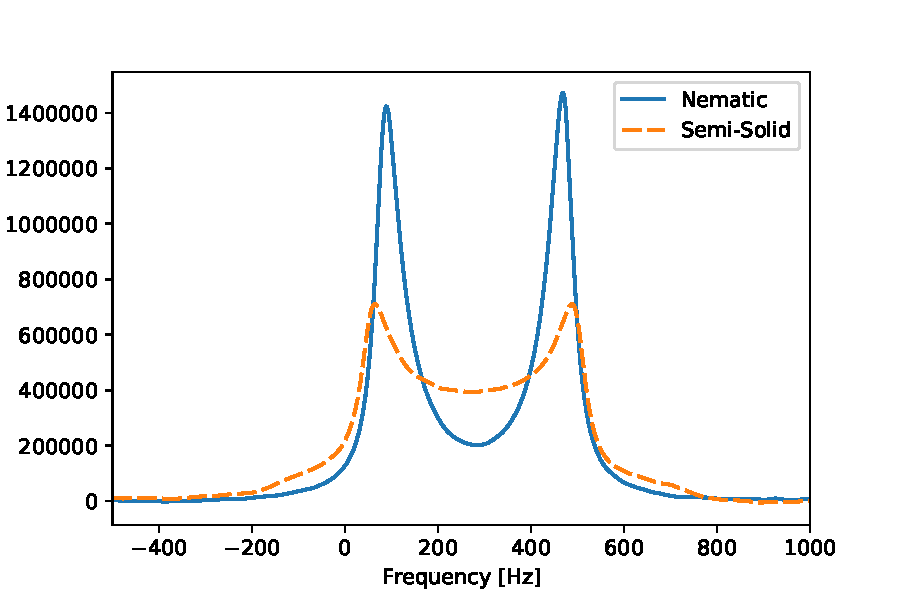
\includegraphics[width=\columnwidth]{nematic_v_semisolid}
  \caption{Comparison between $^2$H-NMR spectra from nematic and semi-solid phases}
  \label{fig:22v23}
\end{figure}

The second maximization step was performed by reducing the amount of SDS used to
prepare each mimetic and subsequently adding phospholipid until a nematic phase
was no longer obtained. The results from the membrane mimetic candidates
prepared in this step are summarized in figure \ref{fig:phase_diag}. From these
preparations, again, the composition with the highest phospholipid content that
retained a nematic phase was chosen for further experimentation. The exact
composition of the membrane mimetic are detailed in table \ref{tab:mimetic_composition}

\begin{figure}[h]
\centering
  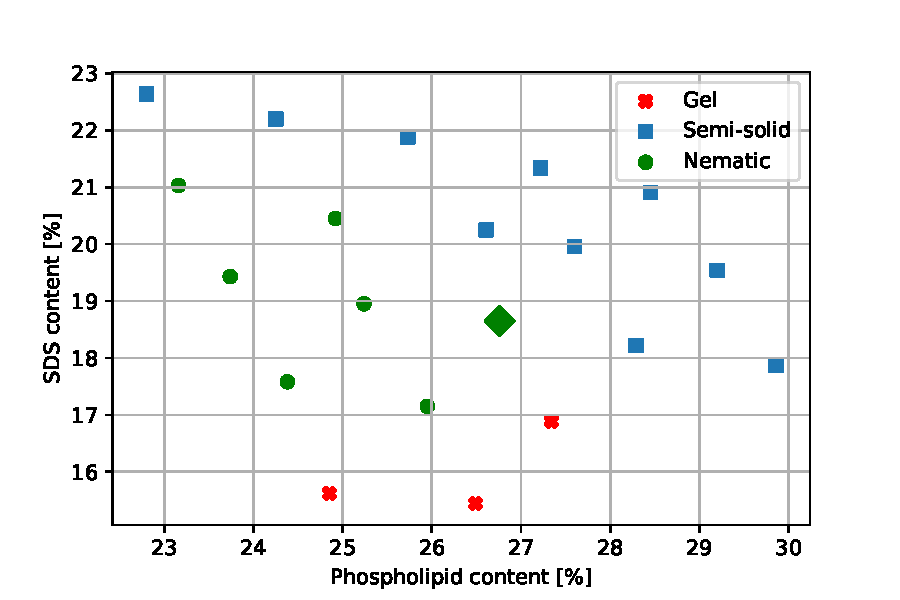
\includegraphics[width=\columnwidth]{phase_diag}
  \caption{Phase diagram of the membrane mimetic when varying SDS and
    phospholipid content. The selected composition is marked as a green diamond.}
  \label{fig:phase_diag}
\end{figure}

\begin{table}[h]
\small
  \caption{\ }
  \label{tab:mimetic_composition}
  \begin{tabular*}{0.48\textwidth}{@{\extracolsep{\fill}}ll}
    \hline
    Compound & Content [$\tfrac{w}{w}\%$] \\
    \hline
    Sodium dodecyl sulphate &  18.65\% \\
    Sodium sulphate & 1.55\%  \\
    1-decanol & 3.92\%  \\
    Phospholipid mixture & 26.76\%  \\
    Water & 49.12\% \\
    \hline
  \end{tabular*}
\end{table}

\section{Calibration of a computational model}
\label{sec:calib}

In order to obtain significant information from a molecular dynamic simulation,
it has to be calibrated to reproduce known experimental results. \par As a first
step, three force-fields with different partial charge distributions were
tested. These force-fields were chosen due to their ability to reproduce
structures of SDS aggregates\todo{citar Tang. et al}.\par
The force-fields tested were:
\begin{itemize}
\item CHARMM36\todo{citar charmm36}
\item Berger with partial charge distribution according to a Merz-Kollman
  method\todo{citar el método MK}
\item Berger with partial charge distribution according to Gromos53A6
  parameters.
\item Gromos53A6 with partial charge distribution according to a Merz-Kollman
  method. And
\item Gromos 53A6 with partial charge distribution according to its own parameters.
\end{itemize}

All simulations were performed using the GROMACS-2016\todo{citar gromacs}
software bundle. A cutoff scheme was used for non-bonding interactions according
to each force-field recommendation values. Temperature control was achieved with
a modified Berendsen thermostat\todo{citar a berendsen}, while pressure was
equilibrated with a semi-isotropic Berendsen barostat. Both temperature and
pressure were adjusted to \SI{310}{K} and \SI{1}{bar} respectively.\\
Before each production simulation, a short equilibration run was performed for a
duration of \SI{1}{ns} with an integration time-step of \SI{1}{fs}. Afterwards,
each production run was calculated to a duration of \SI{40}{ns} with an
integration time-step of \SI{2}{fs}. TIP3P water model was employed on the
simulation with CHARMM36 force-field, while SPC/E was employed on simulations
with Berger and Gromos53A6 force-fields. The same initial configuration was
employed to test each force-field, and it was generated using the software
Packmol\todo{citar packmol} arranging a bilayer with composition in the same
proportion as the membrane mimetic in table \ref{tab:mimetic_composition} to a
total of 9613 molecules. The phospholipid mixture was simulated as a mixture of
39\% PLPC, 26\% DLPC, 24\% DLPE and 11\% DOPE. These proportions were chosen in
accordance with the composition of the phospholipid mixture employed.\\

From each resulting simulation run, order parameters ($S_{CD}$) were calculated
from the SDS aliphatic chain, which were used to calculate a predicted qudrupolar
splitting employing equation \ref{eq:splitting} which depends on a coupling
constant ($e^2qQ/h$) and the angle ($\theta$) between the normal to the bilayer and the
applied magnetic field.

\begin{equation}
  \label{eq:splitting}
  \Delta\nu = \frac{3}{4} \frac{e^2qQ}{h}(3\cos^2\theta - 1) S_{CD}
\end{equation}

These predicted qudrupolar splittings were compared with experimental results,
as shown in figure \ref{fig:calibration}, concluding that employing the
Gromos53A6 force-field yields the results that are closer to experimental
ones, yielding a good correlation on the carbons closer to the interface and
diverging towards the interior of the bilayer.

\begin{figure}[h]
\centering
  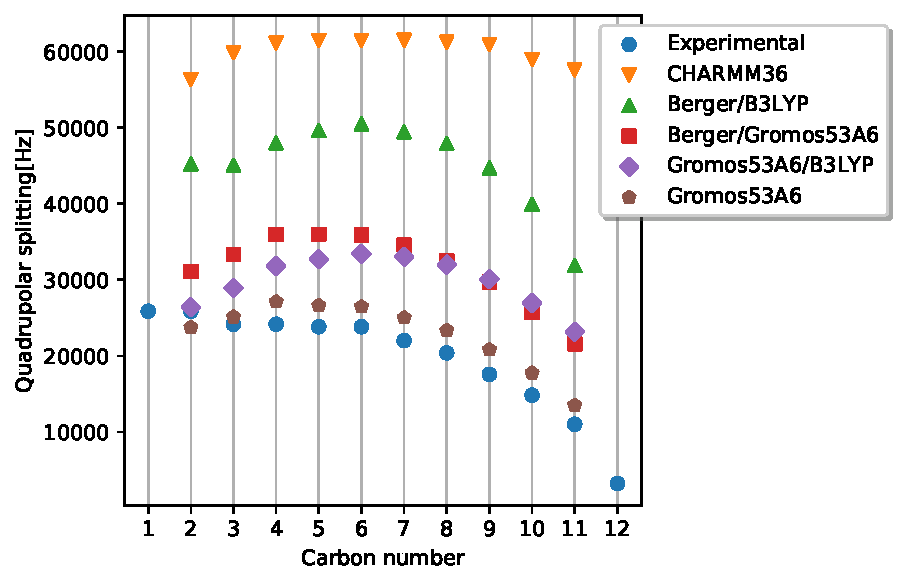
\includegraphics[width=\columnwidth]{calibration}
  \caption{Quadrupolar splittings of SDS-d$_{25}$ from a $^2$H-NMR. Comparison
    between experimental results and predicted by molecular dynamics employing
    different force-fields}
  \label{fig:calibration}
\end{figure}

Further improvement was done to the fitting of predicted results by employing
two thermostats in the simulation, one governing the bulk solution with a
reference temperature of \SI{310}{K} and another governing the bilayer
components with a reference temperature of \SI{320}{K}. The reasoning behind
this decision was based on the expectation that the increased velocity on the
bilayer components would have a further effect on the mobility towards the
center on the bilayer rather than in the interface, where Coulombic interactions
are stronger and have a restraining effect on the mobility of the bilayer. After
this adjustment, the simulation results in predicted quadrupolar splittings in
very good agreement with the experimental ones, as shown in figure
\ref{fig:2nd_calibration}.

\begin{figure}[h]
\centering
  \includegraphics[height=3cm]{example1}
  \caption{Quadrupolar splittings of SDS-d$_{25}$ from a $^2$H-NMR. Comparison
    between experimental results and predicted by molecular dynamics with
    symmetric and asymmetric thermostat}
  \label{fig:2nd_calibration}
\end{figure}

\section{Membrane mimetic validation}
\label{sec:validation}

In order to corroborate that the composition achieved (table
\ref{tab:mimetic_composition}) behaves as a membrane mimetic, we tested the
permeation properties of two drugs: Benzocaine, that is known to be able to passively
cross the cellular membrane; and Levodopa, which is known to be able to cross the
cellular membrane via active mechanisms, therefore it should not be able to
permeate a membrane mimetic without specific receptors.

\subsection{Benzocaine control}
\label{sec:benzo}

\begin{figure*}[h]
\centering
  \includegraphics[height=3cm]{example1}
  \caption{Mean force potential profile for the process of Benzocaine
    translocating through a membrane mimetic.}
  \label{fig:benzocaine_profile}
\end{figure*}
Employing the calibrated model stated before, a potential of mean force (PMF)
profile was calculated for the process of Benzocaine permeating the membrane
(figure \ref{fig:benzocaine_profile}) employing the Umbrella
Sampling/WHAM\todo{citar el método WHAM} method. From this PMF profile it can be
deduced that Benzocaine goes though three steps in order to complete its
translocation: First, it integrates spontaneously with the outer leaflet of the
bilayer, without mayor interactions with the Stern layer. Secondly, Benzocaine
``flip-flops'' to the inner leaflet of the bilayer with a small activation
energy (\SI{11.2}{\kilo\joule}). And third and finally, it escapes the bilayer
into the
bulk at a minor energetic cost (\SI{27.1}{kJ}), showing that Benzocaine
permeation through the membrane mimetic is indeed possible.\\
$^2$H-NMR spectum was taken from a membrane mimetic sample with \SI{8}{mg}
Benzocaine added per gram of mimetic enriched with SDS-d$_{25}$, and compared to
a spectrum of the same mimetic without the anesthetic (figure
\ref{fig:sds_benzocaine}). From this result, it can be seen that the presence of
Benzocaine alters the quadrupolar splittings of the SDS aliphatic chain from the
first up to the sixth carbon, implying that Benzocaine is mostly residing in
this area, this is concordant with the results of the PMF profile (figure
\ref{fig:benzocaine_profile}), which shows that the most stable position for the
Benzocaine to be in, is indeed inside the bilayer and closer to the interface.

\begin{figure}[h]
\centering
  \includegraphics[height=3cm]{example1}
  \caption{Variation on quadrupolar splitting upon adding Benzocaine to a
    membrane mimetic sample.}
  \label{fig:sds_benzocaine}
\end{figure}

\subsection{Levodopa control}
\label{sec:ldopa}

Employing the same method as in Benzocaine, a PMF profile was calculated for the
process of Levodopa permeating the membrane mimetic (figure \ref{fig:levodopa_profile})

\begin{figure*}[h]
\centering
  \includegraphics[height=3cm]{example1}
  \caption{Mean force potential profile for the process of Levodopa
    translocating through a membrane mimetic.}
  \label{fig:levodopa_profile}
\end{figure*}

\section{Conclusions}
The conclusions section should come in this section at the end of the article,
before the Conflicts of interest statement.

\section*{Conflicts of interest}
In accordance with our policy on
\href{http://www.rsc.org/journals-books-databases/journal-authors-reviewers/author-responsibilities/#code-of-conduct}{Conflicts
  of interest} please ensure that a conflicts of interest statement is included
in your manuscript here. Please note that this statement is required for all
submitted manuscripts. If no conflicts exist, please state that ``There are no
conflicts to declare''.

\section*{Acknowledgements}
The Acknowledgements come at the end of an article after Conflicts of interest
and before the Notes and references.

%%% END OF MAIN TEXT%%%

% The \balance command can be used to balance the columns on the final page if
% desired. It should be placed anywhere within the first column of the last
% page.

\balance

% If notes are included in your references you can change the title from
% 'References' to 'Notes and references' using the following command:
% \renewcommand\refname{Notes and references}

%%% REFERENCES%%%
\bibliography{rsc} %You need to replace "rsc" on this line with the name of your .bib file
\bibliographystyle{rsc} %the RSC's .bst file

\end{document}
